%%%%%%%%%%%%%%%%%%%%%%%%%%%%%%%%%%%%%%%%%%%%%%%%%
% Relatório Final - Projeto de Pesquisa
% Métodos de Otimização
% Baltz & Machado
% Capítulo 1
%%%%%%%%%%%%%%%%%%%%%%%%%%%%%%%%%%%%%%%%%%%%%%%%%


\chapter{\Large{Métodos Matemáticos de Otimização}}\label{chp:1}


\section{{O Conceito de Otimização}}

\hspace{0.8cm}
Diz-se otimização, o processo que tem como objetivo encontrar condições que
minimizam ou maximizam algo (seja energia, tempo, dinheiro, etc). Sendo este,
muitas vezes um trabalho árduo, custoso.

Dessa maneira, na matemática, tal processo é amplamente utilizado quando
busca-se valores em conjunto um \textit{A} (que pode ter restrições), com o
objetivo de encontrar uma solução ótima (a melhor resposta para o problema),
aplicando os valores de \textit{A} em uma função objetivo predefinida.

Podendo assim, ser representada da forma como a seguir.

Dada uma função
\begin{equation}
    f : A \subseteq \mathbb{R} \rightarrow \mathbb{R}.
\end{equation}


A maximização pode ser definida como; a busca pelo elemento
\(x^* \in A\), que satisfaz:

\begin{equation}
    f(x^*) \geq f(x),
\end{equation}

para todo \(x \in A\).


A minimização pode ser definida como; a busca pelo elemento \(x^* \in A\),
que satisfaz:

\begin{equation}
    f(x^*) \leq f(x),
\end{equation}

para todo \(x \in A\).

\vspace{\baselineskip}
Com isso, podemos agora entender como esse processo pode ser custoso. Iniciando
com o fato de que existem os pontos máximos e mínimos (pontos
críticos\footnote{Iremos denotar como pontos críticos apenas aqueles onde a função tem derivada e esta se anula.}), locais
e globais, na imagem das funções. Sendo os pontos críticos locais, aqueles que
não são os menores ou maiores valores para a minimização e maximização,
respectivamente. E os pontos globais, aqueles que representam o menor ou maior
valor na imagem das funções, para a minimização e maximização, respectivamente.

Criando, desse modo, uma certa incerteza ao encontrar um valor crítico numa função,
já que, é estritamente difícil saber se o ponto crítico encontrado é local ou
global. Como pode-se perceber na Figura
\ref{grafico_local_global_pontosCriticos}.

\begin{figure}[h]
    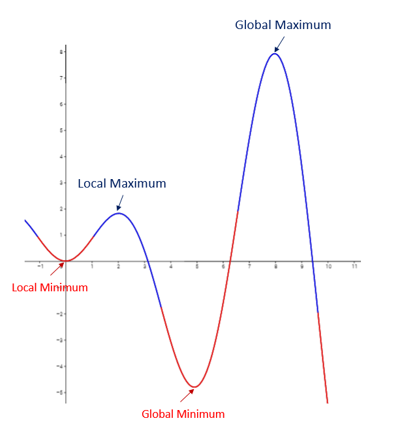
\includegraphics[width=0.43\textwidth]
        {src/grafico_local_global_pontosCriticos.png}
    \centering
    \caption{Exemplo de pontos críticos locais e globais indicados no gráfico
        de uma função.}
    \label{grafico_local_global_pontosCriticos}
\end{figure}

Como na grande maioria dos casos não é possível conhecer antecipadamente todo
o espaço gerado pela função, a busca pelo ótimo pode resultar em pontos
críticos locais. Donde, dependendo do problema, tais resultados chegam a ser
satisfatórios. No entanto, quando o objetivo é estritamente encontrar os máximos
ou mínimos globais, o trabalho necessário acaba sendo mais custoso, pelo fato de
que há a incerteza da existência de mais pontos na grande maioria dos problemas.

Ademais, o conjunto $A$, o qual contém os valores aplicáveis no problema, podem
respeitar restrições, fazendo com que o campo de respostas do problema, não seja
contínuo.

\section{{Otimização de Funções à Uma Variável Real}}

\hspace{0.8cm}

Evidentemente, as funções possuem as variáveis dependentes (que representam o
objeto da otimização) e as variáveis independentes (que suas grandezas podem
ser selecionadas), podemos denotar que, para a equação
\begin{equation}
	y = f(x),
\end{equation}
quando buscamos otimizá-la, temos como objetivo encontrar valores, \(x\), que
quando aplicados à \(f(x)\), temos o mínimo ou máximo valor \textit{y} (seja
ele local, ou preferencialmente, global).

Partindo dessa perspectiva, acaba surgindo a necessidade de utilizar algum
recurso para encontrar os pontos críticos. E nesse sentindo, pode-se utilizar
a técnica de \textbf{derivação}, que oferece o recurso de identificar tais
pontos.


Podemos observar um fator interessante; por exemplo,
quando a função está num ponto máximo, existem duas possibilidades, a primeira,
a função para de crescer e, em seguinda, torna-se indefinida; e a
segunda possibilidade, quando a função para de crescer e começa a decrescer.
Com isso, é importante ressaltar que por definição, quando a derivada (taxa de
variação) em um ponto é positiva, a função cresce, e quando é negativa a função
decresce. Conclui-se que, quando a taxa de variação é zero, a função ou para de
crescer ou de decrescer, o que configura um ponto de máximo ou de mínimo. Mas
também, é quando podo ocorrer o que denominamos ponto de sela (é um
comportamento errático da função, que precisa de uma análise mais refinada). Ou
em última instância, quando a função é constante.

Com o uso da derivada, podemos pensar num método de otimização bastante simples,
considerando \(f(x)\) a função que queremos otimizar e \(f'(x)\) sua função
derivada, podemos dizer que o conjunto $O$, abaixo definido, possui todos os ótimos locais e
globais de \(f(x)\):

\begin{equation}
    O := \{f(x) | f'(x) = 0\}.
    \label{equacao_conjunto_o}
\end{equation}


Portanto, aplicando um filtro em $O$ para obter o máximo e mínimo do conjunto,
acabamos por obter o máximo e mínimo de \(f(x)\):


\begin{equation}
    max(f(x)) = max(O),
\end{equation}

\begin{equation}
    min(f(x)) = min(O).
\end{equation}


Então podemos perceber três problemas:

\begin{itemize}
  \item Determinar como encontrar os pontos onde a derivada se anule, isto é, os pontos críticos;
  \item Determinar se temos de fato todos os pontos;
  \item Classificação dos pontos críticos, que nos revela quais são os máximos e
  os mínimos, e, ademais, da sua relevância quanto a serem locais ou globais.
\end{itemize}

Consideraremos, por agora, apenas o problema de encontrar os pontos críticos.


A taxa de variação de uma função, \(y=f(x)\), em relação a \(x\), é dada pela
relação \(\Delta y / \Delta x\). Sendo o cálculo da derivada
demonstrado pela Figura \ref{derivada_padrao}, o que nos leva ao fato de que
 os pontos críticos provém do conjunto solução da equação \(f'(x) = 0\), como
 definido na equação \ref{equacao_conjunto_o}. Além disso, caso a função esteja
 definida num intervalo fechado, temos pelo Teorema do Valor Absoluto, a
 garantia que ela atingirá o valor dos seus pontos extremos, ou seja, seus
 valores de máximo e mínimo serão atingidos naquele intervalo. O que culmina
 nossa busca pelos pontos críticos.

\begin{figure}[h]
    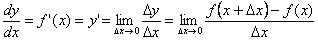
\includegraphics[width=0.45\textwidth]
        {src/derivada_padrao.jpg}
    \centering
    \caption{Derivada: taxa de variação \(dy/dx\).}
    \label{derivada_padrao}
\end{figure}

Partindo desse pressuposto, é nítido que a derivada de uma função é também uma
função. Portanto, fica evidente que uma função pode ser derivada
mais de uma vez, sendo essas derivadas, denominadas de `primeira derivada',
`segunda derivada' e por ai em diante. De modo que, a segunda derivada é
a derivada da primeira derivada. Concluindo-se que dada a função
\(f(x)\), sua primeira derivada é \(df/dx = p(x)\), e sua segunda derivada
\(dp/dx = s(x)\).

Agora vamos tratar da classificação dos pontos críticos.

É sabido que a primeira derivada representa a taxa de variação instantânea de
um ponto na curva, e, que, a segunda derivada proporciona informações
complementares, como por exemplo, se é um ponto de máximo, mínimo ou inflexão,
de modo que, ela determina a concavidade da curva naquele ponto. Como pode ser
visto na Figura \ref{relacao_primeira_segunda_derivada}. E, de modo construtivo,
devemos ressaltar que é importante o estudo do gráfico das derivadas de uma
função, pois é necessariamente através do uso da intrepretação do comportamento
da primeira derivada e/ou da segunda derivada, que obtemos a classificação dos
pontos críticos seguindo os critérios que são apontados na Figura \ref{relacao_primeira_segunda_derivada}.

\begin{figure}[h]
    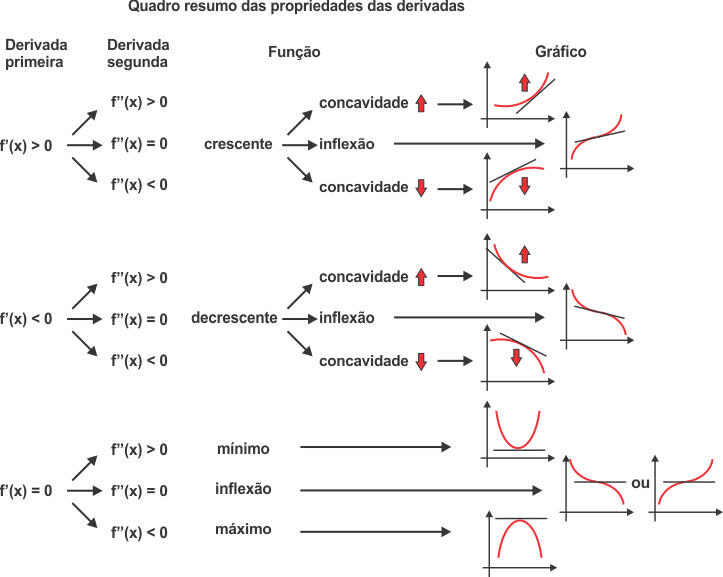
\includegraphics[width=0.65\textwidth]
        {src/relacao_primeira_segunda_derivada.jpg}
    \centering
    \caption{Propriedades e relação da primeira e segunda derivada.}
    % TODO:
    % \tiny Essa imagem foi coletada de \href{https://www.alfaconnection.pro.br}}
    \label{relacao_primeira_segunda_derivada}
\end{figure}


\section{{Programando o Método}}

\hspace{0.8cm}


A própria definição da derivada já nos oferece uma visão simples de como
ela pode ser implementada num programa de computador. Mas, com alguns nuances
que devem ser levados em consideração, segue a tal implementação:


\begin{lstlisting}[]

pub fn derive1x1_v1<F>(f: &F, x: f64) -> f64
where
    F: Fn(f64) -> f64,
{
    (f(x + h) - f(x)) / h
}


\end{lstlisting}


Essa implementação é ingênua no que diz respeito a precisão da operação. O
uso, depende da aplicação, caso se queira prezar por velocidade de cálculo e
muito pouco sobre precisão, então provavelmente, essa solução seja boa o
suficiente. O problema com a precisão desta implementação é que não se é
levado em consideração o aspecto infinitesimal da variação (\(\Delta x\) na
Figura \ref{derivada_padrao}, ou a variável \textit{h} na implementação
em Rust), já que é por este aspecto que definimos a derivada. Não temos como ter
uma variável com tal propriedade num programa de computador. Como consequência,
\(f(x + h) - f(x)\) já é calculada de forma falha, entregando uma variação
diferente da que seria quando se tem uma variável infinitesimal. O que de fato
é entregue, é a variação um pouco mais à frente do ponto esperado.

A partir daí podemos reformular, considerando esse deslocamento, redefinindo
da seguinte forma:


\begin{equation}
    f'(x) = \frac{f(x + h) - f(x - h)}{2h}.
\end{equation}

Que é equivalente à:

\begin{equation}
    f'(x) = \frac{f(x + h) - f(x - h)}{(x + h) - (x - h)}.
\end{equation}


Usaremos essa segunda formulação por motivos de custo de multiplicação de de
números reais se comparado a somas e subtrações, além da possível perda de
precisão. Assim, conseguimos compensar o tal deslocamento numa nova função
insignificantemente mais custosa, e mais precisa. Como vemos no código a seguir:

\begin{lstlisting}[]

pub fn derive1x1_v2<F>(f: &F, x: f64) -> f64
where
    F: Fn(f64) -> f64,
{
    let x1 = x - h;
    let x2 = x + h;

    let y1 = f(x1);
    let y2 = f(x2);
    return (y2 - y1) / (x2 - x1);
}


\end{lstlisting}



\textcolor[rgb]{1,0,0}{\section{{Otimização de Funções à Várias Variáveis}}}

\hspace{0.8cm}





%
